\documentclass[11pt]{article}
% Defining all packages that are used in this document
\usepackage[utf8]{inputenc}
\usepackage[english]{babel} % Change this to norwegian if report is written in norwegian
\usepackage{amsmath}   % Package for math files
\usepackage{parskip}   % No indent, but instead paragraphs
\usepackage{graphicx}  % Place figures
\usepackage{caption}   % Place captions in tables and figures
\usepackage{subcaption}% 
\usepackage{subfiles}  % 
%\usepackage{subfigure}
\usepackage{pdfpages}
\usepackage[T1]{fontenc} 
\usepackage[euler]{textgreek} % To get greek letters as we know them
\usepackage{amssymb}   % 
\usepackage{placeins}  % \FloatBarrier so figures can't float beyond some point in text
\usepackage{fullpage}  % Uses more of the page
\usepackage{float}     % Able to make figures and tables float \begin{figure}[H] to keep them HERE
\usepackage[version=4]{mhchem} % \ce{} to write chemical eq.
\usepackage{siunitx}   % Ex: \si{\meter\per\square\second}
\usepackage{booktabs}  % Behind-the-scenes optimization of tables. \toprule, \midrule, \bottomrule
\usepackage{multirow}
\usepackage{hyperref}  % Ability to click on references like equations, figures, sections etc. \ref{eq:my_eq} clickable

%表格自动生成
\renewcommand {\thetable} {\thechapter{}.\arabic{table}}
%表格根据章节自动命名
\renewcommand {\thefigure} {\thechapter{}.\arabic{figure}}
%图片根据章节自动命名
\numberwithin{figure}{section}
\numberwithin{table}{section}
\numberwithin{equation}{section}
%以上三个皆控制重命名

\usepackage{fontspec}
\setmainfont{Times New Roman}

\hypersetup{
    colorlinks,
    citecolor=black,
    filecolor=black,
    linkcolor=black,
    urlcolor=black
}
\iffalse
\usepackage{fancyhdr}
	%fancyhdr:一个很强大的宏包,用于自定义设计页面风格并命名以供调用。
	\pagestyle{fancy}
	%\rhead{实验B16 基于vLight的光学仿真基础实验}
	%\lhead{基础物理实验\uppercase\expandafter{\romannumeral2}实验报告}
	\cfoot{ \thepage}  %当前页
	\rfoot{\today}
		%分别是右页眉、左页眉、中页脚、右页脚
	\renewcommand{\headrulewidth}{0pt}
	%\renewcommand{\theenumi}{(\arabic{enumi})}
\fi

\usepackage[autolinebreaks,useliterate,numbered]{mcode} % Ability to paste smooth MATLAB code
\newcommand{\figref}[1]{\figurename~\ref{#1}} %Nice reference to figures
%\linespread{1}
\usepackage{setspace}
\setstretch{1.2}
%\renewcommand{\baselinestretch}{1.5}
\title{
    Lift Force on an Aerofoil  \\
    (lab experiment)}
\author{
	Jiaqi, Yao%
    \footnote{jy431@exeter.ac.uk}
}
%\date{  \today}

\begin{document}
\maketitle
%\begin{abstract}
\setlength{\parindent}{2em}
%\end{abstract}
\pagenumbering{gobble} % Turn off page numbering
%\newpage
%\tableofcontents
%\newpage
\pagenumbering{arabic} % Turn on normal pagenumbering
%%%%%%%%%%%%%%%%%%%%%%%%%%%%%%%%%%%%%%%%%%%%%%%%%%%%%%%%%%
% Main contents - Do NOT write your text in main.tex! Use                     the tex files in the folders below
\section{Outline}
\FloatBarrier % Now figures cannot float above section title

In this laboratory experiment, the focus is on determining the lift force acting on an aerofoil using the Air Flow bench in a vertical wind tunnel. By examining the pressure distribution across the aerofoil's surface at varying angles of attack, the experiment aims to relate this pressure to the overall lift produced by the aerofoil.



\section{Theory}
\FloatBarrier % Now figures cannot float above section title

Lift on an aerofoil is crucial for aircraft elevation, which can be interpreted by the Coanda effect and the different pressures between top and bottom surfaces. 

For a symmetric aerofoil at zero angle, the lift generated is zero. 
After increasing the angle of the aerofoil, the pressure variability and producing more lift. 

However, at significant angles, the airflow over the top of the wing can detach due to boundary layer effects, altering the pressure distribution and resulting in lower lift coefficients.This phenomenon is known as "stalling".
The experimental setup is shown in the \autoref{demo}.
\begin{figure}[htbp] % Here, top, bottom priority list
    \centering
    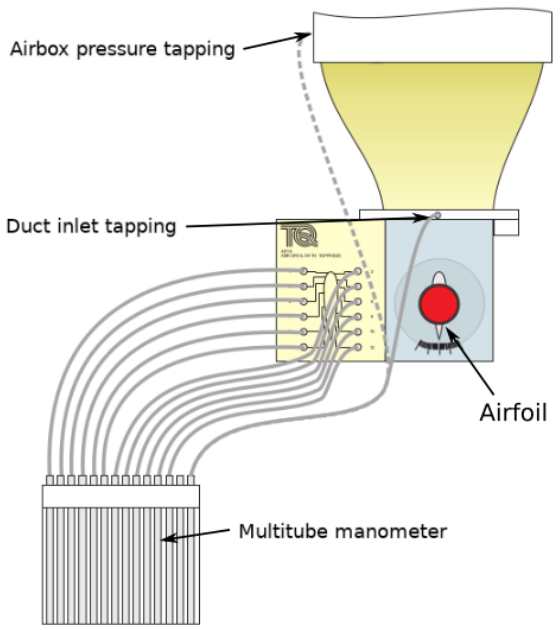
\includegraphics[scale=0.3]{fig/AF18.png}
    \caption{Pressure tappings for AF18 Experiment}
    \label{demo}
\end{figure}

\section{Method}
\FloatBarrier % Now figures cannot float above section title

a. An accurate value for the density of air was determined using room temperature and atmospheric pressure, as cited in Rogers and Mayhew (1992 pp.157-8).

b. With the aerofoil positioned at a 0° angle of attack, pressure measurements were recorded.

c. The effective static pressure should be computed by using the atmospheric and duct inlet pressures.

d. Using the effective static pressure ($P_{eff}$) and the airbox pressure reading, calculate the free stream velocity and determined the Reynolds number with chord length. 

e. For each pressure tapping reading, the corresponding value of pressure ratio($C_{p,n}$) was calculated, and these values were plotted against ($\frac{x}{c}$). The curves were extended to represent a chord ratio of 0 and 1. Noticed that the pressure coefficient near the leading edge is approaching zero, which indicate the directing of the air is disappeared at this point. The exact position of this stagnation point changes with incident angle.

f. From the generated curves of $C_p$, the lift coefficient ($C_L$)can be numerically integrated to derive its value.

g. The measurements have been repeated for increasing angles of attack (in steps of $5^\circ$) up to $25^\circ$, with additional measurements at $17.5^\circ$ and $22.5^\circ$.
Following this, the lift coefficients were computed and a graph illustrating $C_L$ vs. $\alpha$ for the aerofoil was plotted.
\section{Results}
\FloatBarrier % Now figures cannot float above section title

The density of mercury and air and atmospheric pressure at this time can be determined from the thermometers ($23.5^\circ$) and manometers($754mmHg$).

The air and mercury densities are ($1.2kg/m^3$and $13.534\times10^3 kg/m^3$) and the atmospheric pressure is ($100107.4792Pa$), as shown by equation $P_a=\rho_{Hg} gh$ and by consulting the density - temperature table of mercury.

The following table shows the data recorded from the experiment.

\begin{table}[]
	\resizebox{1\textwidth}{!}{
	\begin{tabular}{@{}cccccccccccccccc@{}}
	\toprule
	& 1 & 3 & 5 & 7 & 9 & 11 & 2 & 4 & 6 & 8 & 10 & 12 & Atm & Airbox & Inlet \\ \midrule
	0 & 196 & 158 & 152 & 158 & 167 & 177 & 184 & 156 & 155 & 164 & 170 & 182 & 186 & 244 & 190 \\
	5 & 236 & 195 & 175 & 175 & 178 & 182 & 124 & 118 & 132 & 148 & 168 & 180 & 186 & 244 & 192 \\
	10 & 146 & 220 & 197 & 187 & 188 & 187 & 58 & 88 & 106 & 146 & 164 & 180 & 186 & 244 & 194 \\
	15 & 244 & 235 & 212 & 199 & 194 & 189 & 13 & 54 & 116 & 146 & 166 & 178 & 186 & 244 & 198 \\
	17.5 & 242 & 239 & 217 & 203 & 196 & 190 & 8 & 42 & 119 & 148 & 165 & 178 & 186 & 244 & 200 \\
	20 & 247 & 236 & 217 & 205 & 197 & 190 & 156 & 154 & 154 & 153 & 154 & 158 & 186 & 244 & 210 \\
	22.5 & 248 & 238 & 220 & 209 & 200 & 192 & 164 & 162 & 162 & 160 & 160 & 162 & 186 & 244 & 214 \\
	25 & 247 & 242 & 226 & 217 & 205 & 196 & 172 & 170 & 169 & 168 & 164 & 164 & 186 & 246 & 218 \\ \bottomrule
	\end{tabular}}
	\end{table}
	
\section{Analysis}
\FloatBarrier % Now figures cannot float above section title

\begin{figure}[htb] % Here, top, bottom priority list
    \centering
    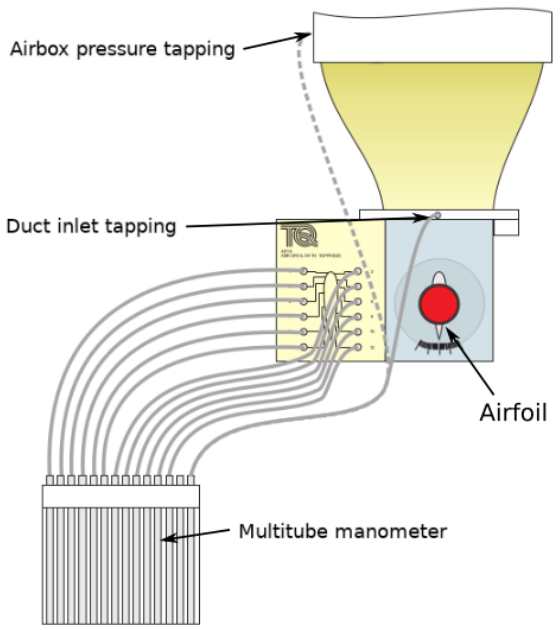
\includegraphics[scale=0.45]{fig/AF18.png}
    \caption{Pressure tappings for AF18 Experiment}
    \label{demo}
\end{figure}


Next the experimental data were processed. Firstly the difference in water head was calculated for each sampling point on tapping position by using the Pitot tube at atmospheric pressure as a standard value. The difference in water head was then converted to a difference in pressure by equation $P_n=\rho gh$, as shown in \autoref{t5.1} below.



% Please add the following required packages to your document preamble:
% \usepackage{booktabs}
\begin{table}[]
    \caption{Preliminary processing of experimental data (Unit: Pa)} 
	\label{t5.1}
    \resizebox{1\textwidth}{!}{
    \begin{tabular}{@{}cccccccccccccccc@{}}\toprule
    Degree/Pitot No.   & 1      & 3       & 5       & 7       & 9       & 11     & 2        & 4        & 6       & 8       & 10      & 12      & Atm & Airbox & Inlet  \\\midrule
    0$^\circ$    & 98.1   & -274.68 & -333.54 & -274.68 & -186.39 & -88.29 & -19.62   & -294.3   & -304.11 & -215.82 & -156.96 & -39.24  & 0   & 568.98 & 39.24  \\
    5$^\circ$    & 490.5  & 88.29   & -107.91 & -107.91 & -78.48  & -39.24 & -608.22  & -667.08  & -529.74 & -372.78 & -176.58 & -58.86  & 0   & 568.98 & 58.86  \\
    10$^\circ$   & -392.4 & 333.54  & 107.91  & 9.81    & 19.62   & 9.81   & -1255.68 & -961.38  & -784.8  & -392.4  & -215.82 & -58.86  & 0   & 568.98 & 78.48  \\
    15$^\circ$   & 568.98 & 480.69  & 255.06  & 127.53  & 78.48   & 29.43  & -1697.13 & -1294.92 & -686.7  & -392.4  & -196.2  & -78.48  & 0   & 568.98 & 117.72 \\
    17.5$^\circ$ & 549.36 & 519.93  & 304.11  & 166.77  & 98.1    & 39.24  & -1746.18 & -1412.64 & -657.27 & -372.78 & -206.01 & -78.48  & 0   & 568.98 & 137.34 \\
    20$^\circ$   & 598.41 & 490.5   & 304.11  & 186.39  & 107.91  & 39.24  & -294.3   & -313.92  & -313.92 & -323.73 & -313.92 & -274.68 & 0   & 568.98 & 235.44 \\
    22.5$^\circ$ & 608.22 & 510.12  & 333.54  & 225.63  & 137.34  & 58.86  & -215.82  & -235.44  & -235.44 & -255.06 & -255.06 & -235.44 & 0   & 568.98 & 274.68 \\
    25$^\circ$   & 598.41 & 549.36  & 392.4   & 304.11  & 186.39  & 98.1   & -137.34  & -156.96  & -166.77 & -176.58 & -215.82 & -215.82 & 0   & 588.6  & 313.92 \\ \bottomrule
    \end{tabular}}
    \end{table}




Based on the \autoref{t5.1}, it was able to calculate the effective static pressure ($p_{eff}$) in different angle by given \autoref{Peff}.
\begin{equation}
    \label{Peff}
   p_{eff}=p_{0}+\frac{85}{135}\times(p_{a}-p_{0})
    \end{equation}
And calculate free stream velocity $U_\infty$ by given \autoref{Uinf} in different angle.
\begin{equation}
    \label{Uinf}
    U_{\infty}={\sqrt{\frac{2\times(p_{airbox}-p_{eff})}{\rho}}}
    \end{equation}
The results are shown in the following \autoref{t5.2}.
% Please add the following required packages to your document preamble:
% \usepackage{booktabs}
\begin{table}[htbp]
    \caption{$p_{eff}$ and $U_\infty$ in different angle(Unit: Pa and m/s)} 
	\label{t5.2}
    \resizebox{1\textwidth}{!}{
    \begin{tabular}{@{}ccccccccc@{}}\toprule
      Pitot No.   & 0        & 5        & 10       & 15       & 17.5     & 20       & 22.5     & 25       \\\midrule
    $p_eff$ & 24.70667 & 37.06    & 49.41333 & 74.12    & 86.47333 & 148.24   & 172.9467 & 197.6533 \\
    $U_\infty$ & 30.11847 & 29.77471 & 29.42693 & 28.71875 & 28.35803 & 26.48081 & 25.69155 & 25.52602\\\bottomrule
    \end{tabular}}
    \end{table}

And from \autoref{cpn},
\begin{equation}
    \label{cpn}
    C_{p,n}={\frac{p_n-p_{eff}}{{\frac{1}{2}}\rho u_{\infty}^{2}}}
    \end{equation}
the pressure ratio in different angle can be calculated. Additionally, the tapping position and airfoil chord for the different sampling points can be obtained from the appendix which is in handbook, and the $x/c$ can be calculated.
% Please add the following required packages to your document preamble:
% \usepackage{booktabs}
\begin{table}[htbp]
    \caption{Pressure ratio in different angle and degree (Unit: Pa)} 
	\label{t5.3}
    \resizebox{1\textwidth}{!}{
    \begin{tabular}{@{}ccccccccccccc@{}}\toprule
    Pitot No.     & 1      & 3      & 5      & 7      & 9      & 11     & 2      & 4      & 6      & 8      & 10     & 12     \\
    $x/c$     & 0.016  & 0.071  & 0.175  & 0.317  & 0.510  & 0.698  & 0.032  & 0.119  & 0.230  & 0.413  & 0.603  & 0.794  \\\midrule
    0    & 0.135  & -0.560 & -0.613 & -0.505 & -0.342 & -0.162 & -0.036 & -0.541 & -0.559 & -0.397 & -0.288 & -0.072 \\
    5    & 0.852  & 0.110  & -0.203 & -0.203 & -0.148 & -0.074 & -1.143 & -1.254 & -0.996 & -0.701 & -0.332 & -0.111 \\
    10   & -0.850 & 0.585  & 0.208  & 0.019  & 0.038  & 0.019  & -2.417 & -1.850 & -1.510 & -0.755 & -0.415 & -0.113 \\
    15   & 1.000  & 0.913  & 0.515  & 0.258  & 0.159  & 0.059  & -3.430 & -2.617 & -1.388 & -0.793 & -0.396 & -0.159 \\
    17.5 & 0.959  & 1.019  & 0.630  & 0.346  & 0.203  & 0.081  & -3.619 & -2.928 & -1.362 & -0.773 & -0.427 & -0.163 \\
    20   & 1.070  & 1.103  & 0.723  & 0.443  & 0.256  & 0.093  & -0.699 & -0.746 & -0.746 & -0.769 & -0.746 & -0.653 \\
    22.5 & 1.099  & 1.223  & 0.842  & 0.570  & 0.347  & 0.149  & -0.545 & -0.594 & -0.594 & -0.644 & -0.644 & -0.594 \\
    25   & 1.025  & 1.340  & 1.004  & 0.778  & 0.477  & 0.251  & -0.351 & -0.401 & -0.427 & -0.452 & -0.552 & -0.552\\\bottomrule
    \end{tabular}}
    \end{table}

Based on \autoref{t5.3}, Pressure distributions are plotted as a graph of the pressure ratio, which at 8 different angles with $x/c$ as the x-axis and $C_p$ as the y-axis.
\begin{figure}
    \centering
    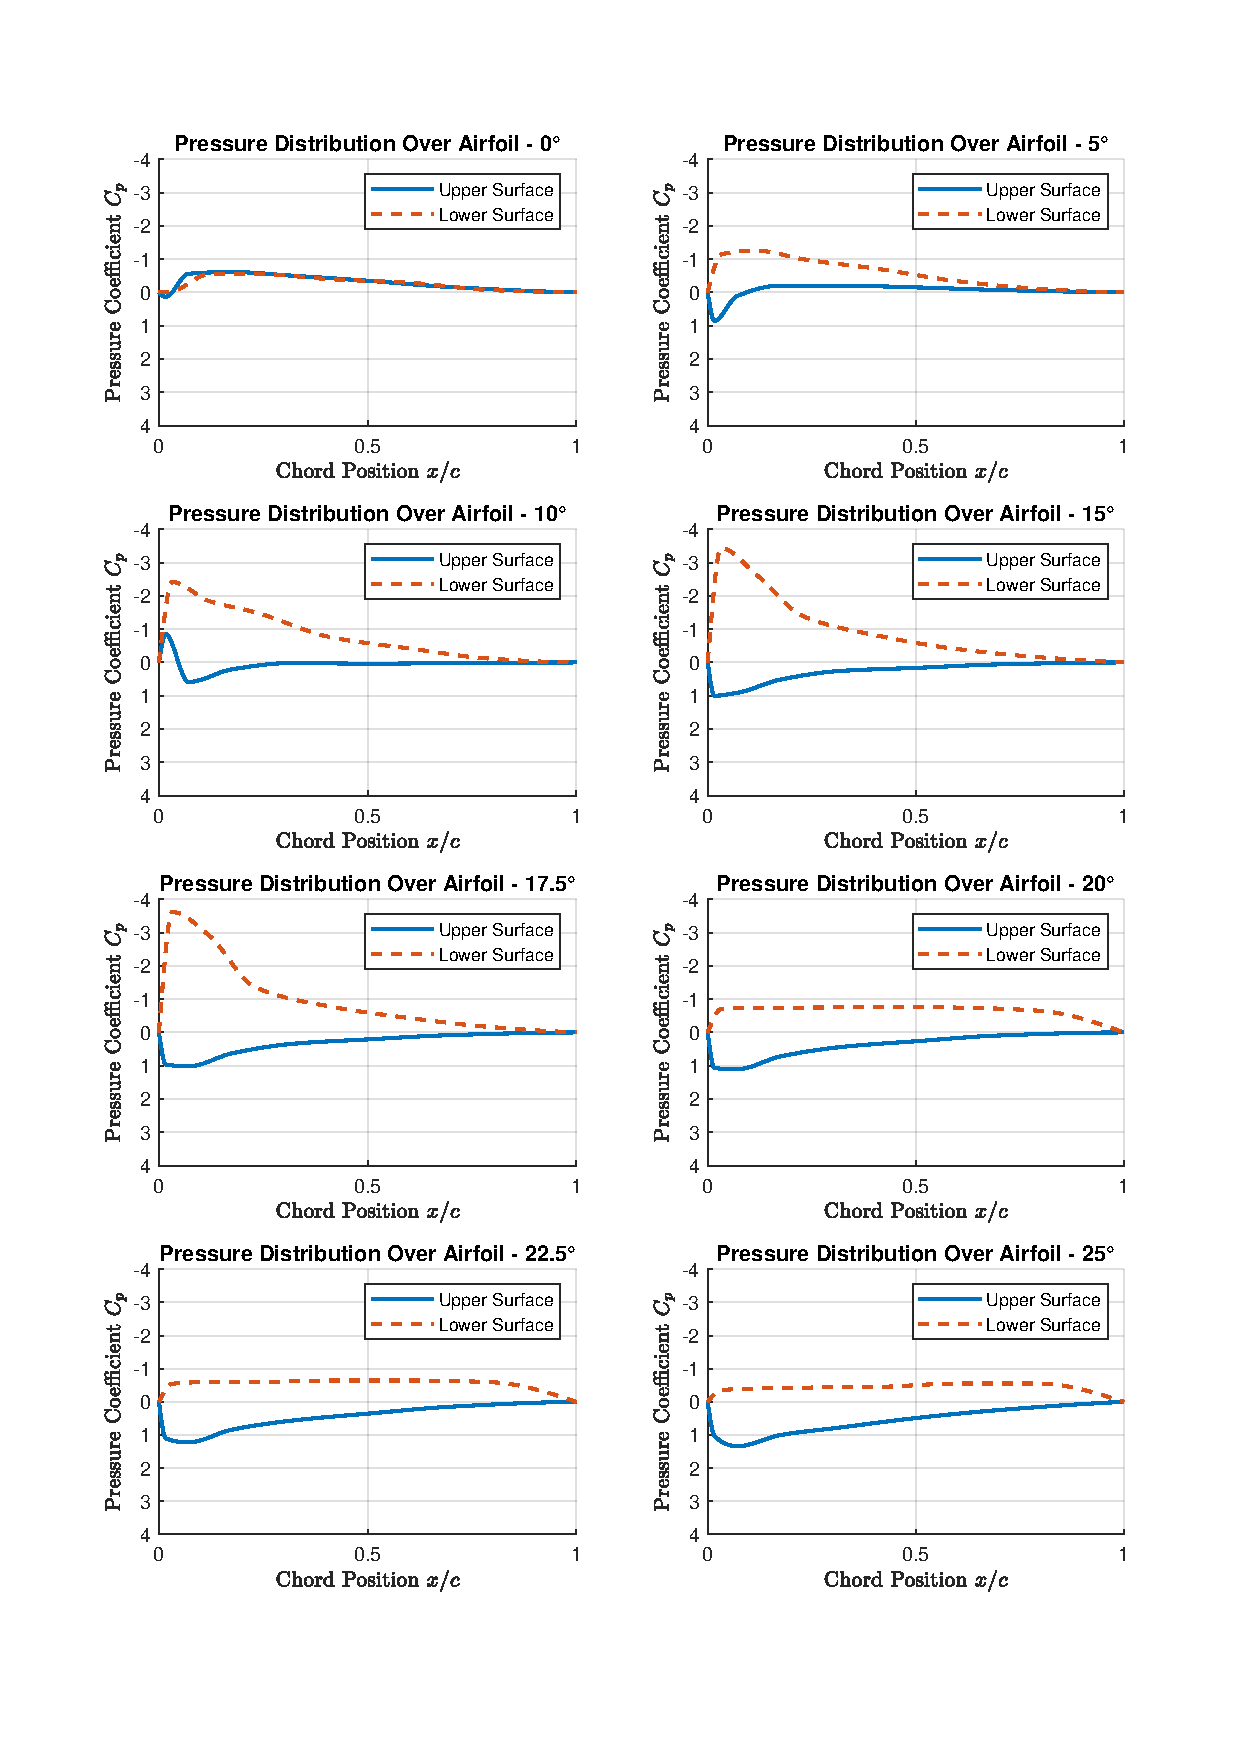
\includegraphics[width=1.05\textwidth]{output.pdf}
    \caption{Pressure distribution over airfoil}
    \label{cp}
  \end{figure}


By using the $C_L$ formular, We can calculate lift coefficient $C_l$.

$$
C_{L}={\frac{F_{L}}{{\frac{1}{2}}\rho U^{2}A}}
$$

Noticed that A is the plan area of the aerofoil. By using mathematical method this can be evaluated by given equation:

$$
C_{L}=\int\left[C_{p l}\left(\frac{x}{c}\right)-C_{p u}\left(\frac{x}{c}\right)\right]d\left(\frac{x}{c}\right)
$$

However, an important point to note is that a direct integration requires a continuous function. In order to find the solution, we use discrete data points to evaluate the $C_L$ by using \textbf{trapezoidal rule}. So, the discrete version of the integral becomes:

$$
\Delta C_{L}=\sum\left(\frac{C_{pl,i+1}+C_{pl,i}}{2}-\frac{C_{p u ,i+1}+C_{p u ,i}}{2}\right)\left(x_{i+1}-x_{i}\right)
$$
Where $i$ is the index of the data points. The results show in a table below.

\begin{table}[]
    \resizebox{1\textwidth}{!}{
    \begin{tabular}{@{}ccccccccc@{}}\toprule
     Degree    & 0        & 5        & 10       & 15       & 17.5     & 20       & 22.5     & 25       \\\midrule
    $C_L$ & -0.040 & 0.383 & 0.676 & 0.939 & 1.015 & 0.840 & 0.828 & 0.830\\\bottomrule
    \end{tabular}}
    \end{table}

    \begin{figure}[htb] % Here, top, bottom priority list
        \centering
        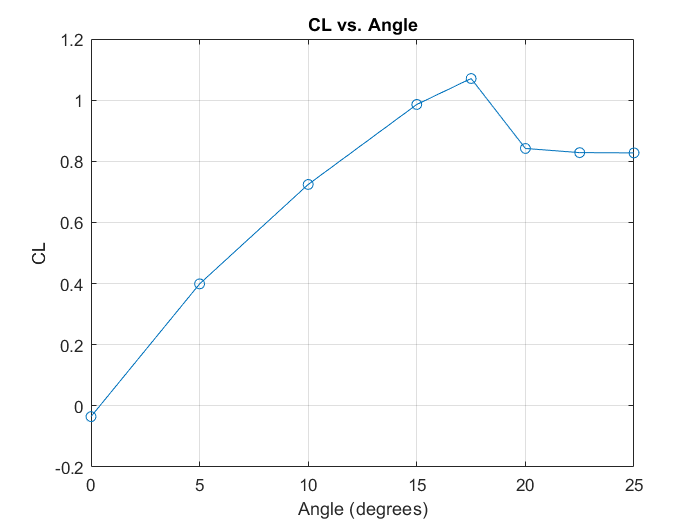
\includegraphics[scale=0.45]{CL.png}
        \caption{Experimental Demonstration}
        \label{fig:demo}
    \end{figure}



\subsection*{Error analysis}



\subsection*{Error analysis}
Error analysis is very important which means the systematic evaluation of the uncertainties or inaccuracies in measurements and calculations, helping to understand the sources and implications of potential deviations from true values.
The possible errors in the experiment are:
\begin{enumerate}
    \item Mercury density and air density are not accurate.
    \item The trapezoidal rule is using discrete point to evaluate the integral, which occur the error.
    \item Pitot tube not sealing well and leaking air.
\end{enumerate}
Some examples of potential errors are given above. The first and third of these are systematic errors and the second is a random error.
Systematic errors can only be improved by improving the accuracy of the measuring equipment. Next, the focus is on analysing the random errors due to the trapezoidal integration method.
The trapezoidal integration method uses a linear connection for integration, which can be optimised by first connecting the discrete points with a smooth curve and then using the different integration method to approximate the true value. The results is in \autoref{t5.5}.    \footnote{The error percentages are calculated based on the values of the Trapezoidal method.}

\begin{table}[htbp]
    \caption{Different integration method to calculate $C_L$}  
    \label{t5.5}
    \centering
    \resizebox{0.8\textwidth}{!}{
    \begin{tabular}{@{}ccccccccc@{}}\toprule
    Degree & 0 & 5 & 10 & 15 & 17.5 & 20 & 22.5 & 25 \\\midrule
    Trapezoidal & -0.040 & 0.383 & 0.676 & 0.939 & 1.015 & 0.840 & 0.828 & 0.830\\
    Simpson's Rule & -0.0206 & 0.4612 & 0.8561 & 1.1218 & 1.2110 & 0.9162 & 0.8964 & 0.8975\\
    Error  (Simpson's) & 48.5\% & 20.4\% & 26.6\% & 19.5\% & 19.4\% & 9.1\% & 8.3\% & 8.1\% \\
    Romberg's method & -0.0228 & 0.4606 & 0.8634 & 1.1261 & 1.2179 & 0.9181 & 0.8989 & 0.9006\\
    Error  (Romberg's) & 43.0\% & 20.3\% & 27.7\% & 19.9\% & 20.0\% & 9.3\% & 8.5\% & 8.5\% \\\bottomrule
    \end{tabular}}
    \end{table}

    \vspace{2cm}
\section{Conclusions}
\FloatBarrier % Now figures cannot float above section title



%\section*{List of Symbols}
\begin{table}[H]
\centering
\begin{tabular}{lll}
 \toprule
  \textbf{Symbol}   &\textbf{Unit}      &\textbf{Explanation}\\
  \midrule
    n               & \si{\mole}        & Amount of substance \\
    m               & \si{\kilo\gram}   & Mass \\
    H               & \si{\kilo\joule\per\mole} & Molar enthalpy \\
    S               & \si{\joule\per\kelvin\per\mole}   & Molar entropy \\
    G               & \si{\kilo\joule\per\mole} & Gibbs free energy \\
    A               & \si{\kilo\joule\per\mole} & Helmholtz free energy \\
  \bottomrule
  \end{tabular}
\end{table}

%%%%%%%%%%%%%%%%%%%%%%%%%%%%%%%%%%%%%%%%%%%%%%%%%%%%%%%%%%
% Bibliography
%\newpage
%\bibliographystyle{IEEEtran}
%\bibliography{mendeley.bib}
%%%%%%%%%%%%%%%%%%%%%%%%%%%%%%%%%%%%%%%%%%%%%%%%%%%%%%%%%%
% Appendix
%\appendix
%\pagenumbering{roman}
%\section{First Appendix}
\label{app:first_appendix}
%\section{Second Appendix}
%\section{Third Appendix}
\end{document}
